


\section{Example}
\label{sec:example}


Next we show a real example database for a time series data. Actual
data come from a temperature distributed sensor monitoring system
\cite{alippi10}, we focus on one sensor data. We use Pytsms and
RoundRobinson implementations in order to create a \acro{MTSDB} and
to query it.

\emph{Data}. The Figure~\ref{fig:exemple:original} shows the original
data for one year and a half. The plot interpolates linearly the
measures. In this plot we can see that there are missing data and some
outlying observations. There are $146\,709$ stored values.

\begin{figure}[tp]
  \centering
  %\tikzset{every picture/.style={scale=0.8}}
  %\tikzsetnextfilename{fig_exemple_original}
  %\usetikzlibrary{dateplot}    
\begin{tikzpicture}
    \begin{axis}[
        date coordinates in=x,
%        xticklabel={\pgfcalendar{tickcal}{\tick}{\tick}{\pgfcalendarshorthand{m}{.}}},
        xticklabel={\pgfcalendarmonthshortname{\month} \year},
        xticklabel style= {rotate=15,anchor=east},
        xlabel=Time,
        ylabel=Temperature (K),
        ymax = 320,
        clip=false,
        y filter/.code = { \pgfmathparse{(#1>320)*322+(#1<320)*#1}},
        ]
       \addplot[blue] file {dades/matriu0.originalbyday.dat};

%      \node[right] at (axis cs:2011-10-12,330) {\footnotesize(2938)};
       \node (break) at (axis cs:2011-10-02,318)[inner sep=0pt,minimum width=0.75em, minimum height=0.5ex,fill=white] {};
    \draw [fill=red,color=blue] (break.north east) -- (break.north west) (break.south west) -- (break.south east);



  \end{axis}
\end{tikzpicture}



%%% Local Variables:
%%% TeX-master: "../main"
%%% ispell-local-dictionary: "british"
%%% End:

  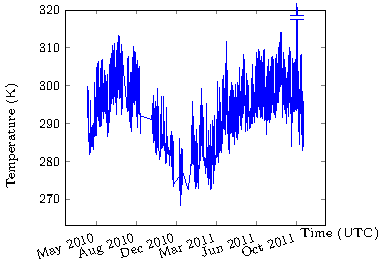
\includegraphics{fig_exemple_original.pdf}
  \caption{Example of a temperature time series data}
  \label{fig:exemple:original}
\end{figure}

\emph{Schema}. We design a \acro{MTSDB} that stores a multiresolution
time series with high resolution at recent times and with low
resolution at older times. The schema is illustrated in the
Figure~\ref{fig:exemple:window}. At the top there are four discs with
different number of measures and at the bottom there is a timeline
showing the resolution subseries along time. Going from most to least
granularity, disks are configured as follows: (i) a measure every 5 h
in the fourth disc which has a capacity of 24 measures and thus it
spans 5 days; (ii) a measure every 2 days in the third disc, with a
capacity of 20 thus spanning 40 days; (iii) a measure every 15 days in
the second disc, with a capacity of 12 thus spanning 180 days and;
(iv) a measure every 50 days in the first disc that, with a capacity
of 12 results in a span of 600 days. This last span is longer than the
original time series so that at least one resolution keeps some data
along the complete original time interval. 

\begin{figure}[tp]
  \centering
  \setlength{\unitlength}{1.3mm}
  %%mrd.afegeix_disc(h5,24,mitjana,zero)
%mrd.afegeix_disc(d2,20,mitjana,zero)
%mrd.afegeix_disc(d15,12,mitjana,zero)
%mrd.afegeix_disc(d50,12,mitjana,zero)
\tiny
\begin{center}
%\begin{multicols}{4} 


    \begin{picture}(14,12)(-7,-6)
    \put(0,-1){\makebox(0,0)[c]{{\color{blue}50 days}}}
      \put(0,0){\circle{10}}
      \put(5,0){\circle{0.8}}
      \put(4.33,2.5){\circle{0.8}}
      \put(2.5,4.33){\circle{0.8}}
      \put(0,5){\circle{0.8}}
      \put(-2.5,4.33){\circle{0.8}}   
      \put(-4.33,2.5){\circle{0.8}}
      \put(-5,0){\circle{0.8}}
      \put(-4.33,-2.5){\circle{0.8}}
      \put(-2.5,-4.33){\circle{0.8}} 
      \put(0,-5){\circle{0.8}}
      \put(2.5,-4.33){\circle{0.8}} 
      \put(4.33,-2.5){\circle{0.8}}
      \put(0,0){\vector(0,1){5}}
      \put(0,0){\oval(5,5)[t]}
      \put(-2.5,0){\makebox(0,0)[c]{$\vee$}}
    \end{picture}
%
    \begin{picture}(14,12)(-7,-6)
    \put(0,-1){\makebox(0,0)[c]{{\color{brown}15 days}}}
      \put(0,0){\circle{10}}
      \put(5,0){\circle{0.8}}
      \put(4.33,2.5){\circle{0.8}}
      \put(2.5,4.33){\circle{0.8}}
      \put(0,5){\circle{0.8}}
      \put(-2.5,4.33){\circle{0.8}}   
      \put(-4.33,2.5){\circle{0.8}}
      \put(-5,0){\circle{0.8}}
      \put(-4.33,-2.5){\circle{0.8}}
      \put(-2.5,-4.33){\circle{0.8}} 
      \put(0,-5){\circle{0.8}}
      \put(2.5,-4.33){\circle{0.8}} 
      \put(4.33,-2.5){\circle{0.8}}
      \put(0,0){\vector(0,1){5}}
      \put(0,0){\oval(5,5)[t]}
      \put(-2.5,0){\makebox(0,0)[c]{$\vee$}}
    \end{picture}
%
    \begin{picture}(14,12)(-7,-6)
    \put(0,-1){\makebox(0,0)[c]{{\color{red}2 days}}}
      \put(0,0){\circle{10}}
      %\put(5,0){\circle{0.8}}
      \put(4.82,1.29){\circle{0.8}}
      \put(4.33,2.5){\circle{0.8}}
     \put(3.5,3.5){\circle{0.8}}
      \put(2.5,4.33){\circle{0.8}}
      \put(1.29,4.82){\circle{0.8}}
      %\put(0,5){\circle{0.8}}
      \put(-1.29,4.82){\circle{0.8}}
      \put(-2.5,4.33){\circle{0.8}}
       \put(-3.5,3.5){\circle{0.8}} 
      \put(-4.33,2.5){\circle{0.8}}
    \put(-4.82,1.29){\circle{0.8}}
      %\put(-5,0){\circle{0.8}}
    \put(-4.82,-1.29){\circle{0.8}}
      \put(-4.33,-2.5){\circle{0.8}}
      \put(-3.5,-3.5){\circle{0.8}} 
      \put(-2.5,-4.33){\circle{0.8 } } 
      \put(-1.29,-4.82){\circle{0.8 }}
      % \put(0,-5){\circle{0.8 }}
     \put(1.29,-4.82){\circle{0.8 }}
      \put(2.5,-4.33){\circle{0.8}}
      \put(3.5,-3.5){\circle{0.8}} 
      \put(4.33,-2.5){\circle{0.8}}
  \put(4.82,-1.29){\circle{0.8}}
      \put(0,0){\vector(0,1){5}}
      \put(0,0){\oval(5,5)[t]}
      \put(-2.5,0){\makebox(0,0)[c]{$\vee$}}
    \end{picture}
%
    \begin{picture}(14,12)(-7,-6)
    \put(0,-1){\makebox(0,0)[c]{{\color{cyan}5 hours}}}
      \put(0,0){\circle{10}}
      \put(5,0){\circle{0.8}}
      \put(4.82,1.29){\circle{0.8}}
      \put(4.33,2.5){\circle{0.8}}
     \put(3.5,3.5){\circle{0.8}}
      \put(2.5,4.33){\circle{0.8}}
      \put(1.29,4.82){\circle{0.8}}
      \put(0,5){\circle{0.8}}
      \put(-1.29,4.82){\circle{0.8}}
      \put(-2.5,4.33){\circle{0.8}}
       \put(-3.5,3.5){\circle{0.8}} 
      \put(-4.33,2.5){\circle{0.8}}
    \put(-4.82,1.29){\circle{0.8}}
      \put(-5,0){\circle{0.8}}
    \put(-4.82,-1.29){\circle{0.8}}
      \put(-4.33,-2.5){\circle{0.8}}
      \put(-3.5,-3.5){\circle{0.8}} 
      \put(-2.5,-4.33){\circle{0.8 } } 
      \put(-1.29,-4.82){\circle{0.8 }}
\put(0,-5){\circle{0.8 }}
     \put(1.29,-4.82){\circle{0.8 }}
      \put(2.5,-4.33){\circle{0.8}}
      \put(3.5,-3.5){\circle{0.8}} 
      \put(4.33,-2.5){\circle{0.8}}
  \put(4.82,-1.29){\circle{0.8}}
      \put(0,0){\vector(0,1){5}}
      \put(0,0){\oval(5,5)[t]}
      \put(-2.5,0){\makebox(0,0)[c]{$\vee$}}
    \end{picture}


%\end{multicols}

\vspace{-10pt}

\setlength{\unitlength}{900sp}
\begin{picture}(14460,5066)(7322,-7148)
\thinlines
{\color[rgb]{0,0,0}\put(7300,-6271){\line( 0,-1){386}}
}%
{\color[rgb]{0,0,0}\put(7782,-6271){\line( 0,-1){386}}
}%
{\color[rgb]{0,0,0}\put(8263,-6271){\line( 0,-1){386}}
}%
{\color[rgb]{0,0,0}\put(8745,-6271){\line( 0,-1){386}}
}%
{\color[rgb]{0,0,0}\put(9227,-6271){\line( 0,-1){386}}
}%
{\color[rgb]{0,0,0}\put(9709,-6271){\line( 0,-1){386}}
}%
{\color[rgb]{0,0,0}\put(10191,-6271){\line( 0,-1){386}}
}%
{\color[rgb]{0,0,0}\put(10673,-6271){\line( 0,-1){386}}
}%
{\color[rgb]{0,0,0}\put(11155,-6271){\line( 0,-1){386}}
}%
{\color[rgb]{0,0,0}\put(11637,-6271){\line( 0,-1){386}}
}%
{\color[rgb]{0,0,0}\put(12119,-6271){\line( 0,-1){386}}
}%
{\color[rgb]{0,0,0}\put(12600,-6271){\line( 0,-1){386}}
}%
{\color[rgb]{0,0,0}\put(13082,-6271){\line( 0,-1){386}}
}%
{\color[rgb]{0,0,0}\put(13564,-6271){\line( 0,-1){386}}
}%
{\color[rgb]{0,0,0}\put(14046,-6271){\line( 0,-1){386}}
}%
{\color[rgb]{0,0,0}\put(14528,-6271){\line( 0,-1){386}}
}%
{\color[rgb]{0,0,0}\put(15010,-6271){\line( 0,-1){386}}
}%
{\color[rgb]{0,0,0}\put(15492,-6271){\line( 0,-1){386}}
}%
{\color[rgb]{0,0,0}\put(15974,-6271){\line( 0,-1){386}}
}%
{\color[rgb]{0,0,0}\put(16456,-6271){\line( 0,-1){386}}
}%
{\color[rgb]{0,0,0}\put(16938,-6271){\line( 0,-1){386}}
}%
{\color[rgb]{0,0,0}\put(17419,-6271){\line( 0,-1){386}}
}%
{\color[rgb]{0,0,0}\put(17901,-6271){\line( 0,-1){386}}
}%
{\color[rgb]{0,0,0}\put(18383,-6271){\line( 0,-1){386}}
}%
{\color[rgb]{0,0,0}\put(18865,-6271){\line( 0,-1){386}}
}%
{\color[rgb]{0,0,0}\put(19347,-6271){\line( 0,-1){386}}
}%
{\color[rgb]{0,0,0}\put(19829,-6271){\line( 0,-1){386}}
}%
{\color[rgb]{0,0,0}\put(20311,-6271){\line( 0,-1){386}}
}%
{\color[rgb]{0,0,0}\put(20793,-6271){\line( 0,-1){386}}
}%
{\color[rgb]{0,0,0}\put(21275,-6271){\line( 0,-1){386}}
}%
{\color[rgb]{0,0,0}\put(7300,-6271){\line( 0,-1){1157}}
}%
{\color[rgb]{0,0,0}\put(9709,-6271){\line( 0,-1){1157}}
}%
{\color[rgb]{0,0,0}\put(12119,-6271){\line( 0,-1){1157}}
}%
{\color[rgb]{0,0,0}\put(14528,-6271){\line( 0,-1){1157}}
}%
{\color[rgb]{0,0,0}\put(16938,-6271){\line( 0,-1){1157}}
}%
{\color[rgb]{0,0,0}\put(19347,-6271){\line( 0,-1){1157}}
}%
{\color[rgb]{0,0,0}\put(21756,-6271){\line( 0,-1){1157}}
}%
{\color[rgb]{0,0,0}\put(7300,-6271){\line( 1, 0){14456}}
}%

\put(7322,-6271){\line( 0,1){3000}}
\put(21756,-7783){\makebox(0,0)[b]{now}}%
\put(7322,-7783){\makebox(0,0)[b]{600 days back}}%

\color{blue}
\put(21782,-5928){\line( -1,0){14460}}
\put(21782,-5928){\line( 0,1){779}}
\put(21782,-5149){\line( -1,0){14460}}
\put(7322,-5928){\line( 0,1){779}}
\put(14530,-5450){\makebox(0,0)[c]{600 days}}

\color{brown}
\put(21782,-5149){\line( 0,1){779}}
\put(21782,-4370){\line( -1,0){4438}}
\put(17344,-5149){\line( 0,1){779}}
\put(19563,-4800){\makebox(0,0)[c]{180 days}}

\color{red}
\put(21782,-4370){\line( 0,1){779}}
\put(21782,-3591){\line( -1,0){964}}
\put(20818,-4370){\line( 0,1){779}}
\put(21300,-3950){\makebox(0,0)[c]{40d}}

\color{cyan}
\put(21782,-3591){\line( 0,1){779}}
\put(21782,-2812){\line( -1,0){120}}
\put(21661,-3591){\line( 0,1){779}}
\put(21300,-3201){\makebox(0,0)[c]{5d}}
\end{picture}%


\normalsize

\end{center}
  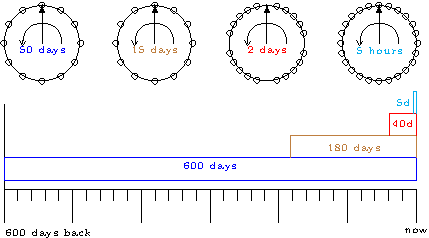
\includegraphics{fig_exemple_window.pdf}
  \caption{Schema of multiresolution}
  \label{fig:exemple:window}
\end{figure}

\emph{Attribute aggregate functions}.  In order to illustrate this
example we consolidate all the resolution subseries using the
mean$^\zohe{}$ aggregate function and the two highest resolution
subseries using the maximum$^\zohe{}$ aggregate function. 



\emph{Consolidation}. The time subseries after consolidating the
\acro{MTSDB} are shown in the Figure~\ref{fig:exemple:4mrd}, where
each graphic corresponds to the possible $\seriedisc$ queries, that is
every resolution disc time series from the \acro{MTSDB}. Each title
shows the resolution subseries and its cardinal, and each attribute
aggregate function has different colour.  Each time series is plotted
with \zohe{} representation function $S(t)^\zohe{}$. Time axis has
\acro{UTC} units rounded to nearest time points and temperature axis
has Kelvin units. Outlayers are marked as discontinuities, for
instance see fourth plot's 2938 K maximum.

\begin{figure}[tp]
  \centering
  % \tikzset{
  %   every picture/.style={scale=0.7},
  % }
  % 
  \begin{tikzpicture}[scale=0.6, every node/.style={transform shape}]
    \begin{axis}[
        multiresoluciodate,
        title={$R_1$: 5h $|24|$},
        xticklabel={\day--\hour:\minute},
        clip=false,
        ]
       \addplot[const plot mark right, blue] table[col sep=comma] {imatges/exemple/dades-matriu0/R18000mean_zohe.csv};
     \node[left] at (axis cs:2011-10-19,274) {\footnotesize oct.~2011};
  \end{axis}
\end{tikzpicture}
%
  \begin{tikzpicture}[scale=0.6, every node/.style={transform shape}]
    \begin{axis}[
        multiresoluciodate,
        title={$R_2$: 2d $|20|$},
        xticklabel={\day~\pgfcalendarmonthshortname{\month}},
        clip=false,
        ]
       \addplot[const plot mark right, blue] table[col sep=comma] {imatges/exemple/dades-matriu0/R172800mean_zohe.csv};
     \node[left] at (axis cs:2011-10-21,279) {\footnotesize 2011};
  \end{axis}
\end{tikzpicture}
%
  \begin{tikzpicture}[scale=0.6, every node/.style={transform shape}]
    \begin{axis}[
        multiresoluciodate,
        title={$R_3$: 15d $|12|$},
        xticklabel={\day~\pgfcalendarmonthshortname{\month}},
        y filter/.code = { \pgfmathparse{(#1>320)*330+(#1<320)*#1}},
        ymax = 320,
        clip=false,
        ]

       \addplot[const plot mark right, blue] table[col sep=comma] {imatges/exemple/dades-matriu0/R1296000mean_zohe.csv};

      \addplot[const plot mark right, orange] table[col sep=comma] {imatges/exemple/dades-matriu0/R1296000maximum_zohe.csv};

      \node[right] at (axis cs:2011-10-07,330) {\footnotesize(2938)};
       \node (break) at (axis cs:2011-09-23,325)[inner sep=0pt,minimum width=0.75em, minimum height=0.5ex,fill=white] {};
    \draw [fill=red,color=orange] (break.north east) -- (break.north west) (break.south west) -- (break.south east);

     \node[left] at (axis cs:2011-10-27,273) {\footnotesize 2011};

  \end{axis}
\end{tikzpicture}
%
\begin{tikzpicture}[scale=0.6, every node/.style={transform shape}]
    \begin{axis}[
        multiresoluciodate,
        xticklabel={\pgfcalendarmonthshortname{\month}~\year},
        title={$R_4$: 50d $|12|$},
        xlabel={Temps (UTC)},
%        ylabel={Temperatura (K)},
        ymax = 320,
        clip=false,
%v1.6     restrict y to domain=0:320,
        y filter/.code = { \pgfmathparse{(#1>320)*330+(#1<320)*#1}},
        ]

       \addplot[const plot mark right, blue] table[col sep=comma] {imatges/exemple/dades-matriu0/R4320000mean_zohe.csv};
       \addlegendentry{mitjana};

       \addplot[const plot mark right, orange] table[col sep=comma] {imatges/exemple/dades-matriu0/R4320000maximum_zohe.csv};
       \addlegendentry{màxim};

       \node[right] at (axis cs:2011-10-12,330) {\footnotesize(2938)};
       \node (break) at (axis cs:2011-08-24,325)[inner sep=0pt,minimum width=0.75em, minimum height=0.5ex,fill=white] {};
    \draw [fill=red,color=orange] (break.north east) -- (break.north west) (break.south west) -- (break.south east);

  \end{axis}
\end{tikzpicture}




%%% Local Variables:
%%% TeX-master: "../../main"
%%% End:

  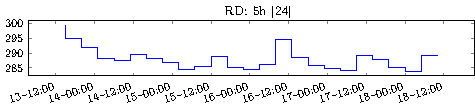
\includegraphics{fig_exemple_4mrd1.pdf}
  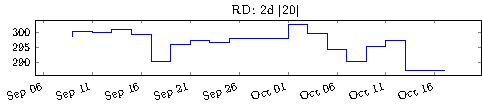
\includegraphics{fig_exemple_4mrd2.pdf}
  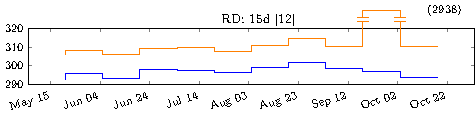
\includegraphics{fig_exemple_4mrd3.pdf}
  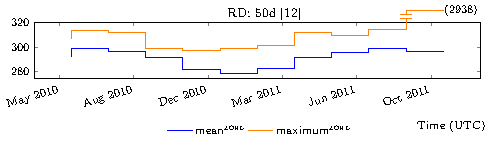
\includegraphics{fig_exemple_4mrd4.pdf}
  \caption{Resolution subseries in the MTSDB}
  \label{fig:exemple:4mrd}
\end{figure}

In all the four plots, we can see that mean aggregate function has
filled missing data and filtered outlayer observations. This is due to
the aggregate function coming from a \zohe{} interpretation.  In the
50 days step resolution, the first data point consolidated is previous
to the original time series. However, it is consolidated with the
first known data as its aggregation comes from \zohe{} interpretation.

Figure~\ref{fig:exemple:4mrdtot} shows the $\totalseries$
queries for the mean$^{\zohe}$ aggregate function resolution and for
the maximum$^{\zohe}$ resolution.  Each resulting time series is
plotted interpolating linearly its measures, note that this linearly
visualisation seems right time displaced as time series comes from a
\zohe{} aggregation.  Comparing this figure with the original series
in Figure~\ref{fig:exemple:original}, we observe that it resembles an
incremental low-pass filter because we applied mean aggregation while
the maximum aggregation resembles an envelope function.

%\tikzsetnextfilename{fig_exemple_4mrdtot}
\begin{figure}[tp]
  \centering
  %\tikzset{every picture/.style={scale=0.8}}
  %\usetikzlibrary{dateplot}  
%\usetikzlibrary{pgfplots.groupplots}

\pgfplotsset{
   petit/.style={
        ylabel=Temperature (K),
%        width=\textwidth,
%        height=3.5cm,
        legend style={font=\footnotesize},
        tick label style={font=\footnotesize},
        label style={font=\tiny},
        title style={font=\small,below, anchor=north,fill=white},
        xticklabel style= {rotate=15,anchor=east},
%        every axis title shift=0pt,
%        max space between ticks=15,
        every mark/.append style={mark size=6},
        major tick length=0.1cm,
        minor tick length=0.066cm,
        very thin,
        every axis legend/.append style={
          at={(1,0.02)},
          anchor=south east,
          draw = none},
        legend columns = 4,
    }
}

\begin{tikzpicture}
    \begin{axis}[
        petit,
        date coordinates in=x,
        xticklabel={\pgfcalendarmonthshortname{\month} \year},
        xlabel=Time (UTC),
%        unbounded coords=jump, %v>1.4
%        unbounded coords=discard, %v>1.4
        ymax = 320,
        clip=false,
%v1.6     restrict y to domain=0:320,
        y filter/.code = { \pgfmathparse{(#1>320)*330+(#1<320)*#1}},
        ]

       \addplot[black!15] file {dades/matriu0.originalbyday.dat};
       \addlegendentry{original};

       \addplot[blue] table[col sep=comma] {dades/mrdb-matriu0/union1.csv};
       \addlegendentry{mean};

       \addplot[orange] table[col sep=comma] {dades/mrdb-matriu0/union0.csv};
       \addlegendentry{max};

%       \node[right] at (axis cs:2011-10-12,330) {\mbox{(2938)}};
       \node (break) at (axis cs:2011-09-25,325)[inner sep=0pt,minimum width=0.9em, minimum height=0.4ex,fill=white] {};
    \draw [fill=red,color=orange] (break.north east) -- (break.north west) (break.south west) -- (break.south east);


  \end{axis}
\end{tikzpicture}
%http://tex.stackexchange.com/questions/46422/axis-break-in-pgfplots

%http://tex.stackexchange.com/questions/52409/insert-a-separate-mark-inside-a-pgfplots-graph



%%% Local Variables:
%%% TeX-master: "../main"
%%% ispell-local-dictionary: "british"
%%% End:

  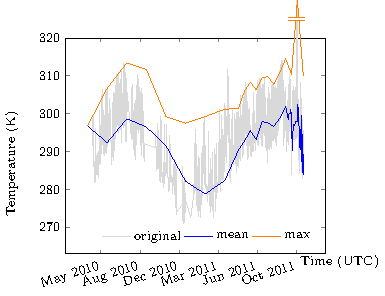
\includegraphics{fig_exemple_4mrdtot.pdf}
  \caption{$\totalseries$ for the mean$^{\zohe}$ and maximum$^{\zohe}$
    resolutions}
  \label{fig:exemple:4mrdtot}
\end{figure}


In conclusion, this \acro{MTSDB} example schema does not store the
complete original data but a compression of the original function
which contains more data for recent times.  Each of the
$\seriedisc$ time series is regular with $\delta$. Although
$\totalseries$ is not a regular time series, it has piece-wise
regularity as a concatenation of every disc's $\delta$.  The purpose
of this example is to show how the multiresolution is computed for a
time series, it has been computed offline as the original data had
already been acquired. However, a \acro{MTSMS} is designed to
consolidate while the original data are being acquired so that the
multiresolution computation spreads along the acquisition and the
computing time becomes less critical.


%%% Local Variables:
%%% TeX-master: "main"
%%% ispell-local-dictionary: "british"
%%% End:

% LocalWords:  multiresolution MTSDB
